\documentclass[12pt]{extarticle}

\usepackage[]{cite}
\usepackage{cmap}
\usepackage[T2A]{fontenc}
\usepackage[utf8]{inputenc}
\usepackage[english, russian]{babel}

\usepackage{tikz}
\usetikzlibrary{matrix}

% latin bold lower
\newcommand{\ba}{\mathbf{a}} 
\newcommand{\bb}{\mathbf{b}}
\newcommand{\bc}{\mathbf{c}} 
\newcommand{\be}{\mathbf{e}} 
\newcommand{\bh}{\mathbf{h}} 
\newcommand{\bp}{\mathbf{p}} 
\newcommand{\bq}{\mathbf{q}}
\newcommand{\bt}{\mathbf{t}} 
\newcommand{\bs}{\mathbf{s}} 
\newcommand{\bu}{\mathbf{u}} 
\newcommand{\bv}{\mathbf{v}} 
\newcommand{\bw}{\mathbf{w}} 
\newcommand{\bx}{\mathbf{x}} 
\newcommand{\by}{\mathbf{y}} 
\newcommand{\bz}{\mathbf{z}} 

% latin bold upper
\newcommand{\bA}{\mathbf{A}} 
\newcommand{\bB}{\mathbf{B}} 
\newcommand{\bC}{\mathbf{C}} 
\newcommand{\bD}{\mathbf{D}} 
\newcommand{\bE}{\mathbf{E}}
\newcommand{\bF}{\mathbf{F}}
\newcommand{\bH}{\mathbf{H}}
\newcommand{\bI}{\mathbf{I}} 
\newcommand{\bJ}{\mathbf{J}}
\newcommand{\bM}{\mathbf{M}} 
\newcommand{\bP}{\mathbf{P}}
\newcommand{\bQ}{\mathbf{Q}}
\newcommand{\bR}{\mathbf{R}}
\newcommand{\bS}{\mathbf{S}}
\newcommand{\bT}{\mathbf{T}} 
\newcommand{\bU}{\mathbf{U}} 
\newcommand{\bV}{\mathbf{V}} 
\newcommand{\bW}{\mathbf{W}} 
\newcommand{\bX}{\mathbf{X}} 
\newcommand{\bY}{\mathbf{Y}} 
\newcommand{\bZ}{\mathbf{Z}} 

% \usepackage{jmlda}
\newcommand{\hdir}{.}
\usepackage{amsmath, amsfonts,amssymb,mathrsfs}
\usepackage{graphicx}
\usepackage{minted}
\usepackage{hyperref}
\usepackage{mathtools}
\usepackage{tocloft}
\usepackage[linesnumbered,boxed]{algorithm2e}
% \usepackage{algorithm}
% \usepackage{algpseudocode}
% \usepackage[usenames]{color}
% \usepackage{colortbl}
\usepackage{setspace}
\doublespacing

\usepackage{graphicx, epsfig}
\usepackage{subfig}
\usepackage{color}

\usepackage{wrapfig}
\usepackage{float}
\usepackage{subfloat}
\usepackage{caption}
\usepackage{multirow}



\newtheorem{theorem}{Теорема}
\newtheorem{lemma}[theorem]{Лемма}
\newtheorem{definition}{Определение}
\newtheorem{remark}{Замечание}
\newenvironment{Proof} % имя окружения
    {\par\noindent{\bf Доказательство.}} % команды для \begin
    {\hfill$\scriptstyle\blacksquare$} % команды для \end

\DeclareMathOperator*{\argmax}{arg\,max}
\DeclareMathOperator*{\argmin}{arg\,min}
\newcommand{\Domain}{\mathcal{D}}
\newcommand{\supp}{\mathrm{supp}}
\newcommand{\diag}{\mathrm{diag}}
\newcommand{\bfw}{\mathbf{w}}
\newcommand{\bfv}{\mathbf{v}}
\newcommand{\bfx}{\mathbf{x}}
\newcommand{\bfz}{\mathbf{z}}
\newcommand{\bfX}{\mathbf{X}}
\newcommand{\bfy}{\mathbf{y}}
\newcommand{\bfb}{\mathbf{b}}
\newcommand{\bbr}{\mathbb{R}}
\newcommand{\bsigma}{\boldsymbol\Sigma}
\newcommand{\expectation}{\mathbb{E}}
\newcommand{\ceil}[1]{\lceil #1 \rceil}

\def\BibAuthor#1{\ruseng{\textit{#1}}}
\def\BibTitle#1{\ruseng{\textrm{#1}}}
\def\BibJournal#1{\ruseng{\textrm{#1}}{\textsl{#1}}}
\def\BibUrl#1{{\small\url{#1}}}
\def\BibHttp#1{{\small\url{http://#1}}}
\def\BibFtp#1{{\small\url{ftp://#1}}}
\def\BibDoi#1{doi:~{\small\url{http://dx.doi.org/#1}}}
\def\typeBibItem{\small\sloppy}

\usepackage[nodisplayskipstretch]{setspace}
\setstretch{1.5}

\textheight=22cm % высота текста
\textwidth=16cm % ширина текста
\oddsidemargin=0pt % отступ от левого края
\topmargin=-1.5cm % отступ от верхнего края
\parindent=24pt % абзацный отступ
\parskip=5pt % интервал между абзацами
\tolerance=2000 % терпимость к "жидким" строкам
\flushbottom % выравнивание высоты страниц

\begin{document}
\thispagestyle{empty}
\begin{center}
    \sc
        «Московский физико-технический институт\\
        \rm{(национальный исследовательский университет)}»\\
        Физтех-школа прикладной математики и информатики\\
        Кафедра <<Интеллектуальные системы>>
        %\\        при Вычислительном центре им. А. А. Дородницына РАН
        \\[25mm]
    \rm\large
        Курдюкова Антонина Дмитриевна\\[10mm]
    \bf\Large
		Снижение размерности фазового пространства в задачах канонического корреляционного анализа\\[10mm]
    \rm\normalsize
        03.03.01 -- Прикладные математика и физика\\[10mm]
    \sc
        Выпускная квалификационная работа бакалавра\\[10mm]
\end{center}
\hfill\parbox{75mm}{
    \begin{flushleft}
    \bf
        Научный руководитель:\\
    \rm
        д.ф.-м.н. Стрижов Вадим Викторович\\[3.9cm]
    \end{flushleft}
}
\begin{center}
    Москва\\
    2022
\end{center}

\newpage
\tableofcontents
\newpage

\begin{abstract}
Данная работа посвящена решению задачи декодирования сигналов и методам сходящегося перекрестного отображения Сугихары. Метод сходящегося перекрестного отображения используется для исследования временных рядов на наличие причинно-следственной связи. С помощью метода PLS, входящего в группу методов канонического корреляционного анализа, можно построить прогноз временного ряда. Современная интерпретация метода Сугихары дает возможность сформулировать важную  гипотезу о том, что метод PLS является частным случаем метода сходящегося перекрестного отображения. 
Сформулирован вариант теоремы о вложениях 
для проверки удовлетворения методов прогноза условиям Сугихары. Решается прикладная задача прогнозирования сигнала гироскопа по сигналу акселерометра при различных типах движения человека
\\
\bigskip
\noindent

\textbf{Ключевые слова}: \emph {снижение размерности, фазовое пространство, аттрактор, метод сходящегося перекрестного отображения, теорема Такенса о вложениях}
\end{abstract}
\newpage

%данные поля заполняются редакцией журнала
% \doi{10.21469/22233792}
% \receivedRus{01.01.2017}
% \receivedEng{January 01, 2017}

% \maketitle

% \cftchapterprecistoc




\section{Введение}


Решается задача прогнозирования сигналов походки человека. Такие сигналы обладают сложной структурой. Под сложной структурой понимается наличие зависимостей и изменяющийся период. Рассматриваются два связанных фазовых пространства. Одно из них является исходным, другое -- целевым. Например, фазовые пространства сигналов акселерометра и гироскопа одного мобильного устройства; пространства сигналов акселерометра в правой руке и акселерометра в левой руке человека; пространство траектории движения руки, восстановленной по видеоряду движения человека, и пространство сигнала акселерометра на этой руке.

Цель работы заключается в построении более простой модели прогнозирования, работающей не хуже уже существующих моделей прогнозирования временных рядов.

Для повышения качества прогноза, а также для упрощения прогностической модели, предлагается учесть зависимости между временными рядами и перейти в пространство меньшей размерности. Снижение размерности позволяет учитывать внутреннее низкоразмерное представление временных рядов. 


Для снижения размерности траекторного пространства используются метод проекций в латентное пространство (partial least squares PLS) \cite{geladi1988notes, hoskuldsson1988pls}. Для этого метода существуют нелинейные модификации, например, описанная в работе \cite{yaushev}. Снижение размерности позволяет сделать прогностическую модель более устойчивой, изучить связь между главными компонентами временных рядов, а также найти траекторное подпространство, в котором обнаружение связи между временными рядами осуществляется наиболее простым путем.

Для определения наличия связи между временными рядами используется метод сходящегося перекрестного отображения (convergent cross mapping, CCM) \cite{sugihara1990nonlinear, sugihara2012detecting}. Метод CCM проверяет, насколько близки точки фазового пространства временного ряда $\by$, соответствующие ближайшим соседям временного ряда $\bx$. Под близостью понимается существование взаимно однозначного соответствия, которое отображает окрестность фазовой траектории $\bx$ в окрестность фазовой траектории $\by$.

В современной литературе описаны различные модификации метода сходящегося перекрестного отображения. Метод симплексной проекции, описанный в \cite{sugihara1990nonlinear}, позволяет строить краткосрочный прогноз траекторий хаотических динамических систем. В работе исследуются различия между детерминированным хаосом системы и ошибкой измерения данных с шумом. Оценивается размерность фазового пространства аттрактора хаотического временного ряда. За рамками статьи остаются временные ряды конечной длины. 
Метод последовательных локально взвешенных глобальных линейных отображений (S-Map), описанный в \cite{sugihara1994nonlinear}, рассматривает временной ряд как результат эволюции динамической системы во времени. Описаны некоторые проблемы, касающиеся прогнозирования при обнаружении нелинейностей и хаоса. Рассматривается нелинейное прогнозирование в задаче классификации. Предлагается метод характеризации нелинейности с помощью S-map и метод анализа нескольких краткосрочных временных рядов сложного аттрактора. В работе \cite{dixon1999episodic} описан метод многомерных вложений. Рассматривается влияние нелинейных процессов на эпизодические взаимосвязи наблюдаемых переменных динамической системы. Подход заключается в построении ряда алгоритмов, от глобального линейного до локального нелинейного, для прогнозирования данных на основе вложений с запаздывающими координатами \cite{rand2006dynamical}. В качестве алгоритма прогнозирования используется метод S-map \cite{sugihara1994nonlinear}.
Подход, описанный в \cite{ye2016information}, применяется к сложным взаимосвязанным системам. Основная идея работы заключается в реконструкции аттрактора многомерного временного ряда с разных точек зрения и их объединение в единую модель. Эффективен для коротких и зашумленных временных рядов.

Метод сходящегося перекрестного отображения используется для исследования временных рядов на наличие причинно-следственных связей. С помощью метода PLS, входящего в группу методов канонического корреляционного анализа, можно построить прогноз временного ряда. Современная интерпретация метода Сугихары дает возможность сформулировать важную  гипотезу о том, что метод PLS является частным случаем метода сходящихся перекрестных отображений.

Требуется построить модель прогнозирования сигналов, включающую в себя метод сходящегося перекрестного отображения и методы канонического корреляционного анализа.

Метод сходящегося перекрестного отображения не предполагает выбора собственного
подпространства, в котором аппроксимируется фазовая траектория временного ряда и не включает
прогностическую модель. В работе \cite{usmanova} выбор собственного подпространства осуществляется перебором по главным компонентам. В работе \cite{Isachenko2021PhDThesis} по PLS представлен метод выбора оптимального подпространства. В данной дипломной работе предлагается перенести методы выбора подпространства с PLS на CCM.\\
Введем несколько базовых понятий.

\textbf{Определение 1.}
\emph{Динамическая система $\mathcal{S}$~--- множество элементов, для каждого из которых задано положение в фазовом пространстве в зависимости от времени.}

Такая математическая модель позволяет изучать различные зависимости, а также изменения систем со временем. 

Динамическая система может описывать различные взаимодействия в природе. Например, связь между сардинами, анчоусами и температурой поверхности моря \cite{sugihara2012detecting}, данные о кори, ветряной оспе и популяции морского фитопланктона \cite{sugihara1990nonlinear}. В данной дипломной работе динамической системой $\mathcal{S}$ является движущийся человек.
  
Динамика различных процессов, в том числе упомянутых выше, не является полностью случайной, то есть изменения динамической системы обладают детерминированностью. Поэтому в основе динамики системы $\mathcal{S}$ лежит \emph{многообразие}\cite{kirby1978manifold} $\bM$, управляющее ей.  
  
\section{Постановка задачи прогнозирования сигнала}
Заданы временные ряды $
 \bx=\{ x_i\}_{i=1}^{N_1}$ и $\by = \{y_i \}_{i=1}^{N_2}. 
$
  Требуется построить прогноз ряда~$\by$ на следующие $m$ значений $N_2+1, \dots, N_2+m$. 
При построении прогностической модели $\mathcal{F}$ нужно учесть влияние ряда $\bx~=~\{ x_i\}_{i=1}^{N_1}$ на ряд $\by$. Значения ряда $\bx$ в моменты времени $N_2+1, \dots, N_2+m$ известны, то есть $N_1 > N_2 + m$.

При построении прогноза ряда $\by$ на один шаг по времени вперед учитываются $h$ предыдущих значений этого ряда и все предшествующие текущему моменту времени значения ряда $\bx$. Тогда прогностическая модель имеет вид:
\begin{equation}
    \widehat{y}\,_{t+1} = \mathcal{F}(\widehat{\mathbf{w}}, y_{t}, \dots, y_{t-L+1}, x_1, \dots, x_t),
    \label{eq:F}
\end{equation}
Решение задачи оптимизации \eqref{eq:optim} дает параметры модели $\bw$:
    \begin{equation}
        \widehat{\mathbf{w}} = \argmin_{\mathbf{w}}\,\mathcal{L}(\mathbf{w}, \by, \widehat{\by}),
    \label{eq:optim}
    \end{equation}
где $\mathcal{L}$~--- функция потерь.

\setlength{\belowdisplayskip}{0pt} \setlength{\belowdisplayshortskip}{0pt}
\setlength{\abovedisplayskip}{5pt} \setlength{\abovedisplayshortskip}{5pt}

\section{Построение прогноза временных рядов}
   Опишем процесс построения фазового пространства $\mathbb{X}$.
   Строится ганкелева матрица~$\bX$ по временному ряду $\bx$:
     \begin{equation}
         \bX = \begin{bmatrix}
                        x_1 & \dots & x_{n} \\
                        x_2 & \dots & x_{n+1} \\
                        \vdots  &\ddots& \vdots \\
                        x_{k_1} & \dots & x_{N_1}
                    \end{bmatrix}^{\mathsf{T}} = 
                    \begin{bmatrix}
                        \bx_1,
                        \bx_2, 
                        \dots,
                        \bx_{k_1}
                    \end{bmatrix}, \quad k_1 = N_1 - n + 1,
                    \label{tr_matrix}
                    \end{equation}\\
где~$n$ -- ширина окна. Тогда вектора $\bx_1, \bx_2, \dots, \bx_{k_1}$ образуют фазовую траекторию или, иными словами, \empf{аттрактор} $\mathbf{M}_X$ временного ряда $\bx$. На эти вектора натянуто фазовое пространство $\mathbb{X}$ размерности $n$. Аналогично, строим ганкелекву матрицу $\bY$ для временного ряда $\by$. Аттрактор $\bM_Y$ и фазовое пространство $\mathbb{Y}$ соответствуют временному ряду $\by$. Формально, под терминами \emph{фазовое пространство} и \emph{аттрактор} будем понимать следующее:

\begin{definition}
Фазовое пространство $\mathbb{X}$ динамической системы $\mathcal{S}$ -- совокупность всех допустимых состояний динамической системы.
\end{definition}


\begin{definition}
Аттрактор $\mathbf{M}$ -- компактное подмножество фазового пространства динамической системы $\mathcal{S}$, описывающее динамику этой системы. 
\end{definition}

\begin{figure}[ht]
\centering
{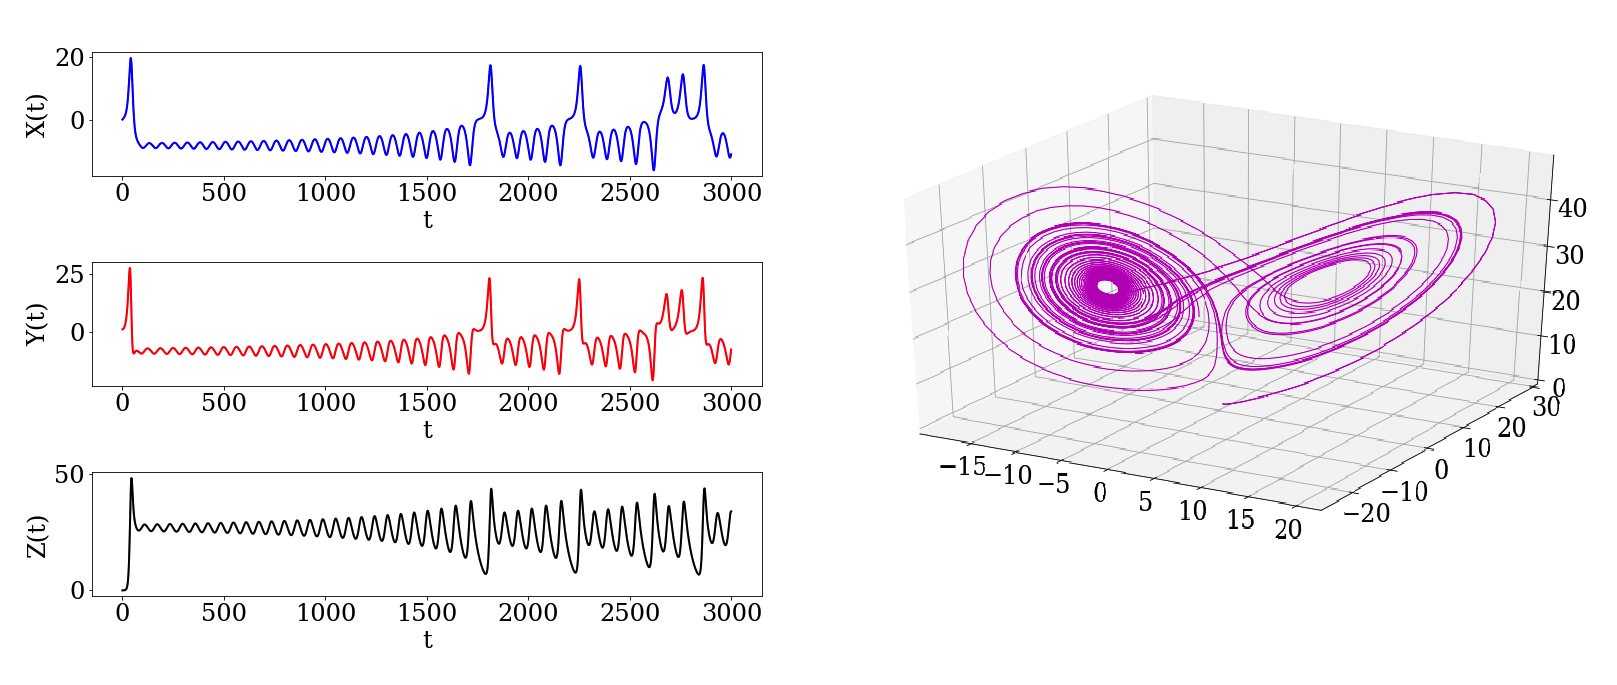
\includegraphics[width=1\textwidth]{./images/ts_xyz.png}}
\caption{Аттрактор Лоренца}
\label{fg:attractor}
\end{figure}

\begin{figure}[ht]
\centering
{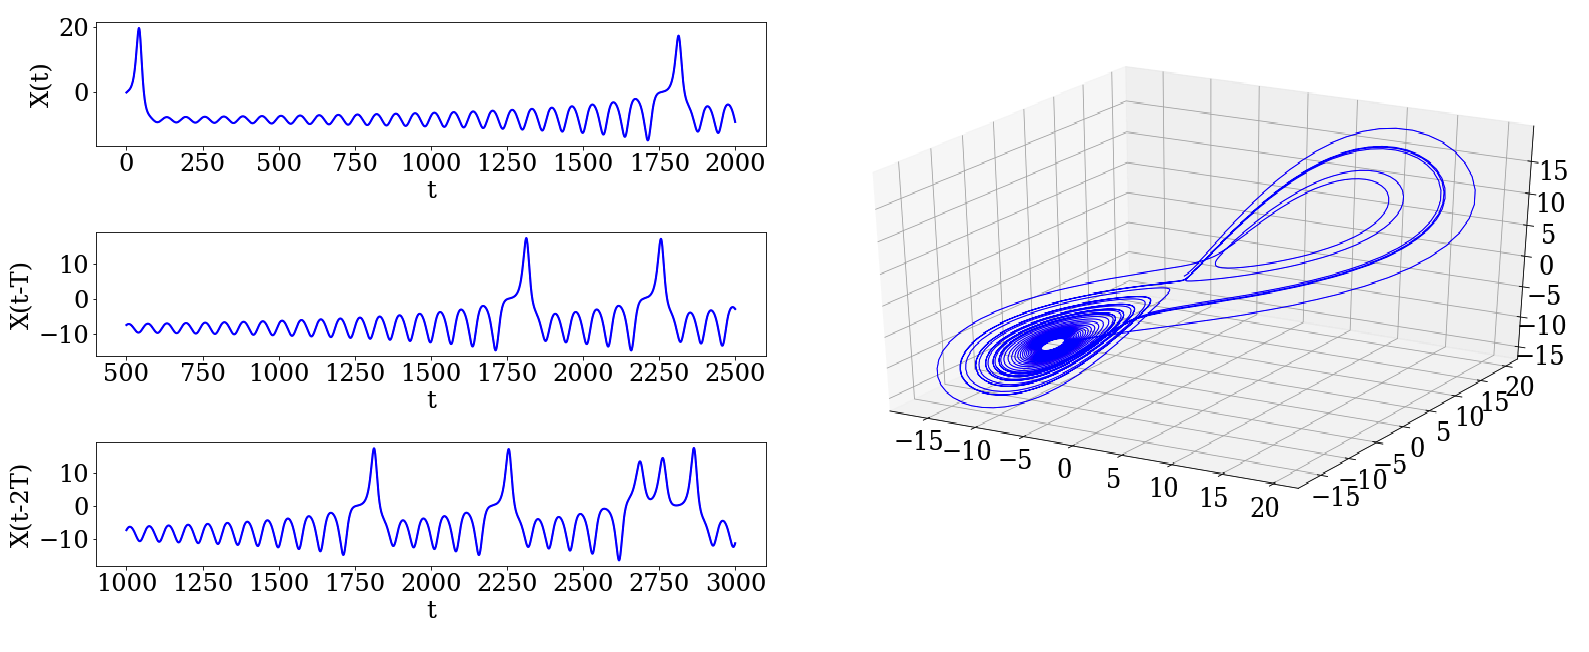
\includegraphics[width=1\textwidth]{./images/attractor_X.png}}
\caption{Аттрактор Лоренца, восстановленный по наблюдаемой X}
\label{fg:attractor_x}
\end{figure}

Одним из способов описания динамической системы является система дифференциальных уравнений, где каждая переменная зависит от состояния и изменения остальных переменных. На рисунке \eqref{fg:attractor} справа в качестве примера представлен аттрактор Лоренца. Динамика описывается системой дифференциальных уравнений:
\begin{equation}
    \begin{cases}
        \dot X = \sigma(Y -X)\\
        \dot Y = X(r - Z) - Y\\
        \dot Z = XY - bZ,
    \end{cases}
    \label{eq:lorenz}
\end{equation}
где $\sigma, \, r,\, b$~--- параметры. Слева на рисунке \eqref{fg:attractor} изображены решения $X(t),\, Y(t),\, Z(t)$ системы дифференциальных уравнений \eqref{eq:lorenz}.
Евклидово пространство данных переменных образует пространство состояний системы. Многообразие состояний системы в этом пространстве образует аттрактор $\mathbf{M}$. Проекция многообразия $\mathbf{M}$ на координатные оси дает временной ряд соответствующей наблюдаемой. С другой стороны, при определенных условиях по временному ряду одной из наблюдаемых можно восстановить многообразие аттрактора в фазовом пространстве. Эти условия описаны в следующем разделе.

\subsection{Теорема Такенса о вложениях}
Теорема Такенса формулирует условия, при которых хаотическая динамическая система $\mathcal{S}$ может быть восстановлена из последовательности наблюдений состояния динамической системы.
Теорему для динамической системы $\mathcal{S}$ с дискретным временем записывается следующим образом:
\begin{theorem}
Пусть $\mathbb{M}$~--- пространство состояний динамической системы $\mathcal{S}$ размерности $\nu$. Динамика системы задается гладким отображением $f_{M}:\: \mathbb{M} \rightarrow~\mathbb{M}$. Предположим, что динамика $f_{M}$ имеет аттрактор $\bM \subset \mathbb{M}$ размерности $d_{M}$. Согласно теореме Уитни о вложениях \cite{whitney1944singularities}, аттрактор $\bM$ может быть вложен в евклидово пространство размерности $d > 2k_M$. То есть, существует диффеоморфизм~$\phi$, который отображает многообразие $\bM$ в пространство $\mathbb{R}^d$, причем производная отображения $\phi$ имеет полный ранг.\\
Диффеоморфизм задается следующим образом:
\begin{equation}
    \phi(x) = (\alpha(x),\, \alpha(f_M(x)),\, \dots,\, \alpha(f_M^{d-1}(x))),
\end{equation}
где $\alpha:\: \bM\rightarrow \mathbb{R}$~--- функция наблюдений, сопоставляет каждой точке аттрактора~$\bM$ вещественное число. Функция $\alpha$ должна быть дважды дифференцируема, а ее производная должна иметь полный ранг.
\label{Taken's theorem}
\end{theorem}
Теорема показывает, что скрытое представление $\mathbf{M}_X$ исходного многообразия $\mathbf{M}$ восстанавливается по одной лишь его проекции, то есть по временному ряду $X(t)$. Теорема проиллюстрирована на рисунке \ref{fg:attractor_x}. Изображен временной ряд $X(t)$ и две его копии $X(t-T)$ и $X(t-2T)$, сдвинутые на интервалы $T$ и $2T$ соответственно. Тогда в координатном пространстве $(X(t),\,X(t-T),\,X(t-2T))$ временные ряды представляют собой скрытое представление $\mathbf{M}_X$ многообразия $\mathbf{M}_X$.

Представление $\mathbf{M}_X$ сохраняет важные математические свойства исходной динамической системы $\mathcal{S}$, которые не меняются при плавном изменении координат. Иными словами, метод позволяет построить \emph{диффеоморфизм} между $\mathbf{M}$ и $\mathbf{M}_X$~--- взаимно однозначное отображение гладких многообразий, причем функция отображения и обратная к ней являются дифференцируемыми. Но геометрическая структура исходного аттрактора $\bM$ при этом не сохраняется.


\subsection{Метод сходящегося перекрестного отображения}
Метод сходящегося перекрестного отображения (convergent cross mapping, CMM) используется для исследования временных рядов на наличие причинно--следственной связи. Корреляция не подразумевает причинно--следственную связь между временными рядами. Метод основан на теореме Такенса о вложениях. В общем случае многообразие аттрактора динамической системы требуется восстановить по одной наблюдаемой.

Согласно принципам метода сходящегося перекрестного отображения временной ряд $\by$ может быть восстановлен по временному ряду $\bx$ только если временной ряд $\bx$ связан с рядом $\by$. Временные ряды считаются связанными, если окрестность фазовой траектории $\bM_{X}$ временного ряда $\bx$ взаимно однозначно отображается в окрестность фазовой траектории $\bM_Y$ ряда $\by$. Иными словами, 

\textbf{Утверждение}
Между аттракторами $\mathbf{M}_X$ и $\mathbf{M}_Y$ существует взаимнооднозначное соответствие $\varphi$, если наблюдаемые $\mathbf{X}$ и $\mathbf{Y}$ принадлежат одной динамической системе.

Построим отображение $\varphi$. Пусть построены ганкелевы матрицы $\bX$ и $\bY$ по временным рядам $\bx$ и $\by$ согласно \eqref{tr_matrix}. Эти матрицы определяют фазовые траектории~$\bM_{X}$ и $\bM_Y$ в фазовых пространствах $\mathbb{X}$ и $\mathbb{Y}$ соответственно. Выберем элемент $\bx_{t_0}$ фазовой траектории $\bM_{X}$. Найдем $k$ ближайших к $\bx_{t_0}$ точек  фазовой траектории $\bM_{X}$. Временные индексы ближайших соседей обозначим $t_1,\dots,t_k$.

Так как временные ряды $\bx$ и $\by$ определены на единой оси времени, то точке\\$\bx_{t_0}\in\bM_X$ взаимно однозначно соответствует точка $\by_{t_0}$ фазовой траектории $\bM_Y$. Аналогично, моментам времени $t_1,\dots,t_k$ однозначно соответствуют точки $\by_{t_1},\dots,\by_{t_k}\in~\bM_Y$.

Отображение $\varphi$ из множества точек $\bM_X$ в $\bM_Y$ введем согласно \cite{pukenas2018algorithm} следующим образом:
\begin{equation}
\varphi: \bx_0 \mapsto \widehat{\by}_0 = \sum\limits_{i=1}^k w_i \by_{t_i}, \qquad 
w_i = \dfrac{u_i}{\sum\limits_{j=1}^k u_j}, \qquad
u_i = \exp \bigl( -||\bx_0 - \bx_{t_i}|| \bigr).
\end{equation}
\begin{definition}
Временные ряды $\bx$ и $\by$ называются \textbf{связанными}, если отображение $\varphi$ является липшицевым:
	$$ \rho_{\mathbb{Y}}(\varphi(\bx_i), \varphi(\bx_j)) \leq C \rho_{\mathbb{X}}(\bx_i, \bx_j), \quad \bx_i, \bx_j \in \bM_X. $$
\end{definition}
Для проверки наличия связи между временными рядами $\bx$ и $\by$ введем метрическую функцию близости векторов в окрестностях $U_k(\bx_{t_0})$ и $U_k(\by_{t_0})$:
\begin{equation}
    J(\bx, \by) = \dfrac{R(U_k(\bx_{t_0}))}{R(U_k(\by_{t_0}))}, \qquad R(U_k(\bx_{t_0})) = \dfrac{1}{k} \sum\limits_{i=1}^k \rho_{\mathbb{X}}(\bx_{t_0}, \bx_{t_j}).
\end{equation}
Если $J(\bx, \by)$ больше заданного порога, то временной ряд $\by$ зависит от временного ряда $\bx$.
\subsection{Метод проекций на латентные структуры}
Метод проекций на латентные структуры PLS~\cite{geladi1988notes, hoskuldsson1988pls} используют для нахождения фундаментальных зависимостей между двумя матрицами $\mathbf{X}$ и $\mathbf{Y}$. Отбираются наиболее значимые признаки. Новые признаки являются линейными комбинациями исходных признаков. Осуществляется переход в фазовое пространство меньшей размерности. Метод PLS позволяет найти фазовое подпространство, в котором наблюдается связь между главными компонентами исходных временных рядов. Это позволяет исследовать наличие связи между временными рядами. 

Пусть $\mathbf{X}\in\bbr^{n\times k_1}$ и $\mathbf{Y}\in\bbr^{n\times k_2}$ ~--- матрицы двух фазовых пространств, построенных по временному ряду $\bx$ и $\by$ соответственно. Требуется построить прогноз временного ряда $\by$ с учетом связи с временным рядом $\bx$. Предполагается линейная зависимость между строками $\mathbf{X}$ и $\mathbf{Y}$:
\begin{equation}
    \mathbf{Y}_i = \mathbf{X}_i\cdot\mathbf{\Theta} + \boldsymbol{\varepsilon}, \quad \mathbf{Y}_i\in\bbr^{k_2},\;\mathbf{X}_i\in\bbr^{k_1},\; i = 1,\ldots,n,
    \label{eq:linear}
\end{equation}
где $\mathbf{\Theta}$ ~--- матрица весов линейной зависимости,\; $\boldsymbol{\varepsilon}$~--- вектор ошибок.

Ошибка вычисляется по формуле:
\begin{equation}
    L(\mathbf{\Theta}, \mathbf{X}, \mathbf{Y}) = \|\mathbf{Y} - \mathbf{X}\cdot\mathbf{\Theta}\|_2^2
    \label{eq:error}
\end{equation}

Алгоритм PLS находит матрицы $\mathbf{T}, \mathbf{U}, \mathbf{P}, \mathbf{Q}$, с помощью которых осуществляется переход в латентное пространство согласно формулам:

\begin{equation}
    \mathbf{X} = \mathbf{T}\cdot \mathbf{P} + \mathbf{F},
\end{equation}
\[
    \mathbf{Y} = \mathbf{U}\cdot \mathbf{Q} + \mathbf{E}.
    \label{eq:latent}
\]
Матрицы $\mathbf{T}, \mathbf{U}$ наилучшим образом описывают $\mathbf{X}$ и $\mathbf{Y}$. Их столбцы ортогональны. Матрицами $\mathbf{P}$ и $\mathbf{Q}$ определяется переход из латентного пространства в исходное. Матрицы $\mathbf{X}$ и $\mathbf{Y}$ ~--- матрицы невязок.

Алгоритм PLS также позволяет определить матрицу $\mathbf{W}$, с помощью которой рассчитывается матрица весов $\mathbf{\Theta}$:
\begin{equation}
    \mathbf{\Theta} = \mathbf{W}(\mathbf{P}^{\mathsf{T}}\mathbf{W})^{-1}\mathbf{Q}^{\mathsf{T}}.
    \label{eq:Q}
\end{equation}

\begin{equation}
		\begin{tikzpicture}
			\matrix (m) [matrix of math nodes,row sep=3em,column sep=3em,minimum width=2em,ampersand replacement=\&]
			{
			    \& \mathcal{S} \&
			    \\
				\mathbf{X}\in\bbr^{n\times k_1} \& \& \mathbf{Y}\in\bbr^{n\times k_2} \\
				\& \mathbf{T}, \mathbf{U} \in \bbr^{n\times\ell} \& \\};
			\path[-stealth]
			(m-1-2) edge [bend right=10] node {} (m-2-1)
			(m-1-2) edge [bend left=10] node {} (m-2-3)
			(m-2-1) edge node [above] {$\mathcal{F}$} (m-2-3)
			(m-2-1) edge [bend right=10] node [below, pos=0.4] {} (m-3-2)
			(m-3-2) edge [bend right=10] node [above, pos=0.4] {$\bP$} (m-2-1)
			(m-2-3) edge [bend left=10] node [below, pos=0.4] {} (m-3-2)
			(m-3-2) edge [bend left=10] node [above, pos=0.4] {$\bQ$} (m-2-3);
		\end{tikzpicture}
\end{equation}

На коммутативной диаграмме $\mathcal{S}$ ~--- динамическая система, порождающая часть, $\mathbf{X} $~--- фазовое пространство, $\mathbf{Y} $~--- наблюдаемое пространство, $\mathcal{F}$ ~--- гомоморфизм, $\mathbf{T}, \mathbf{U}$ ~--- латентно-согласованные пространства, не можем измерить напрямую.

Стоит обратить внимание на прогностическую модель $\mathcal{F}$ и на отображение $\varphi$. Обе функции задают связь между фазовыми пространствами $\mathbb{X}$ и $\mathbb{Y}$. Современная интерпретация метода сходящегося перекрестного отображения позволяет сформулировать следующую гипотезу о связи $\mathcal{F}$ и $\varphi$:

\textbf{Гипотеза}
Метод проекций на латентные структуры является частным случаем метода сходящегося перекрестного отображения.
\newpage
Гипотеза позволяет перенести многие важные факты, справедливые для метода PLS, на метод сходящихся перекрестных отображений.

\section{Вычислительный эксперимент по анализу гипотезы}


\begin{figure}[h!]
\centering
{\includegraphics[width=1.1\textwidth]{./images/acc+gyr_new-2.png}}
\caption{Данные акселерометра и гироскопа одного мобильного устройтсва для ходьбы}
\label{fg:signal}
\end{figure}

\begin{figure}[h!]
\centering
  \subfloat[Акселерометр]{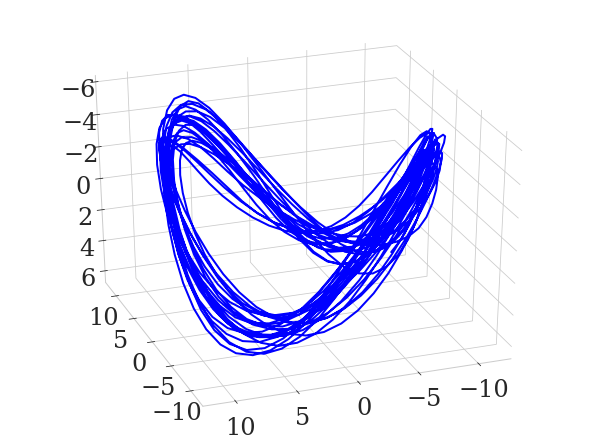
\includegraphics[width=0.6\textwidth]{./images/acc_tr_1_new.png}}
   \hspace{0.5cm}
  \subfloat[Гироскоп]{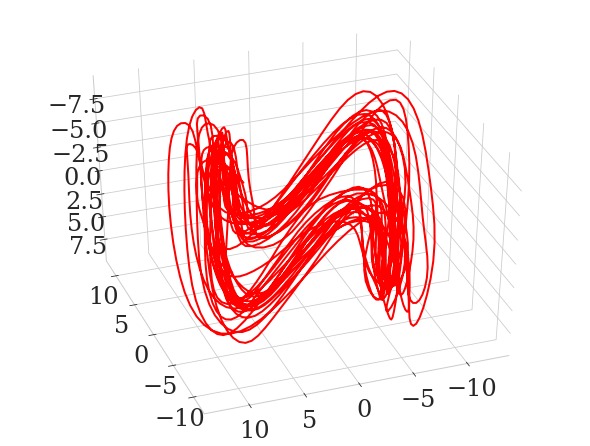
\includegraphics[width=0.6\textwidth]{./images/gyr_tr_1_new.png}}\\
\caption{Траектории в фазовом пространстве для ходьбы}
\label{fg:initial_traj}
\end{figure}


\begin{figure}[h!]
\centering
{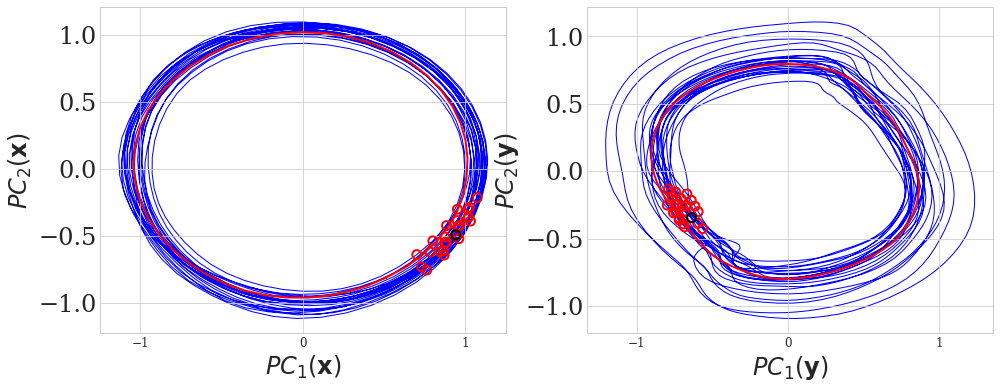
\includegraphics[width=1\textwidth]{./images/knn-2.png}}
\caption{Поиск ближайших соседей на фазовой траектории для метода CCM}
\label{fg:CCM}
\end{figure}


\begin{figure}[h!]
\centering
{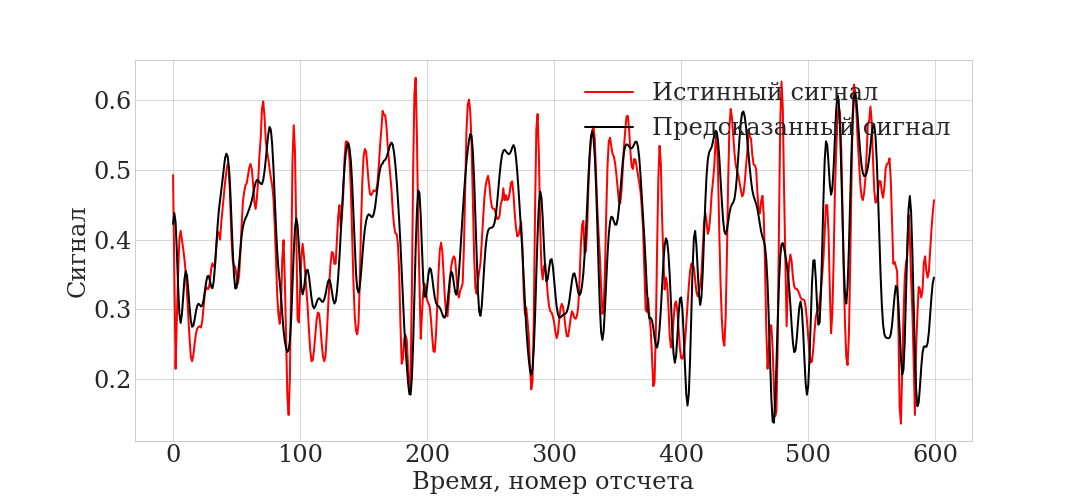
\includegraphics[width=1\textwidth]{./images/corr_new.png}}
\caption{Истинный и предсказанныий с помощью алгоритма PLS сигнал гироскопа для ходьбы}
\label{fg:pred}
\end{figure}

\begin{figure}[h!]
\centering
{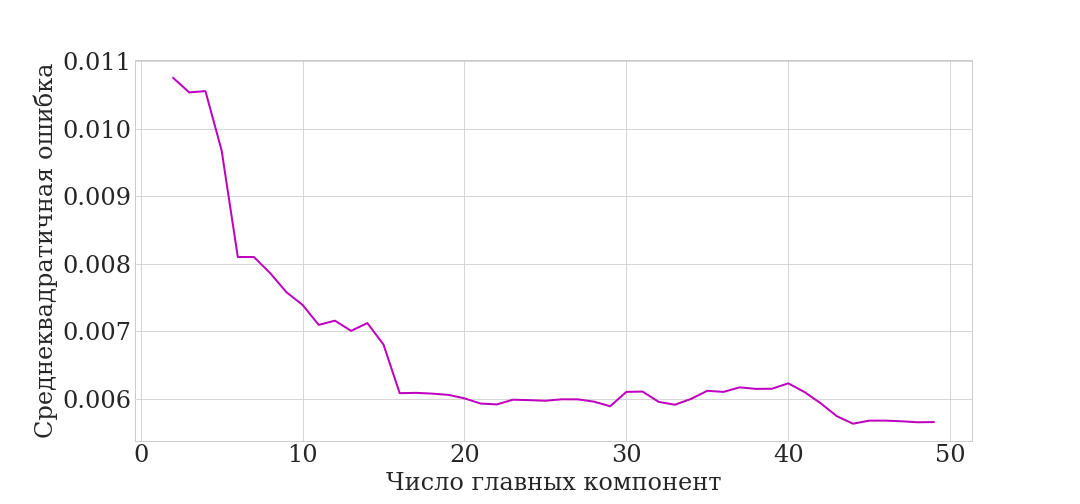
\includegraphics[width=1\textwidth]{./images/ERROR_new.png}}
\caption{Зависимость ошибки MSE прогноза от числа главных компонент для зависимых рядов}
\label{fg:error_corr}
\end{figure}



\begin{figure}[h!]
\centering
{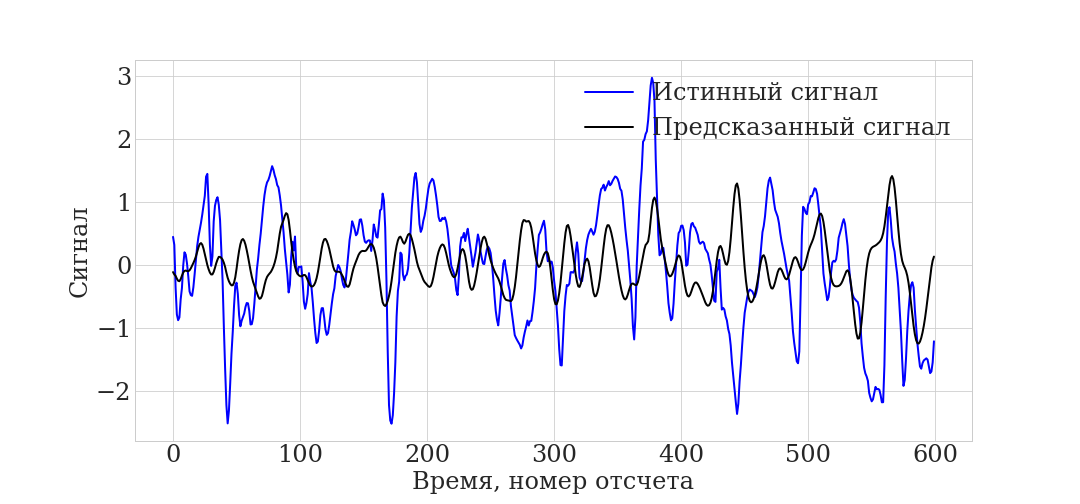
\includegraphics[width=1\textwidth]{./images/uncorr_new.png}}
\caption{Предсказание сигнала акселерометра для несвязанных сигналов с помощью алгоритма PLS}
\label{fg:uncorr}
\end{figure}

\begin{figure}[h!]
\centering
{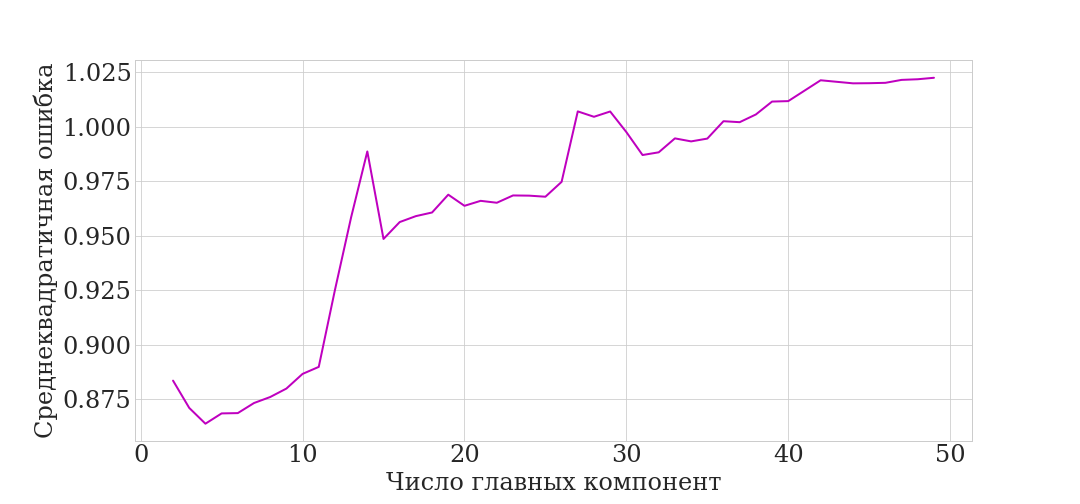
\includegraphics[width=1\textwidth]{./images/ERROR2_new.png}}
\caption{Зависимость ошибки MSE прогноза от числа главных компонент для несвязанных временных рядов}
\label{fg:error_uncorr}
\end{figure}


\begin{figure}[!htbp]
\centering
{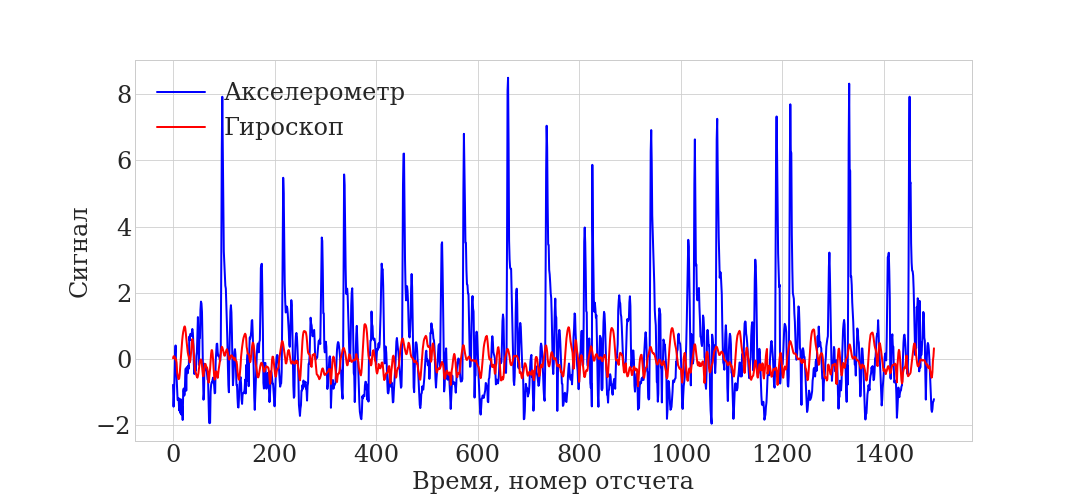
\includegraphics[width=1.1\textwidth]{./images/signal_long_new-2.png}}
\caption{Данные акселерометра и гироскопа одного мобильного устройтсва для медленной ходьбы}
\label{fg:long_signal}
\end{figure}

\begin{figure}[h!]
\centering
  \subfloat[Акселерометр]{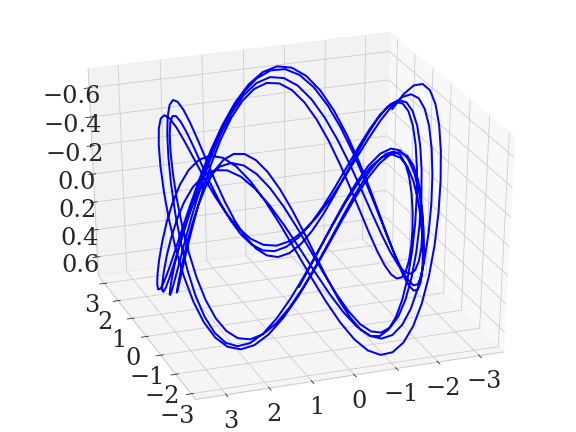
\includegraphics[width=0.6\textwidth]{./images/acc_tr_2_new.png}}
  \wspace{0.5cm}
  \subfloat[Гироскоп]{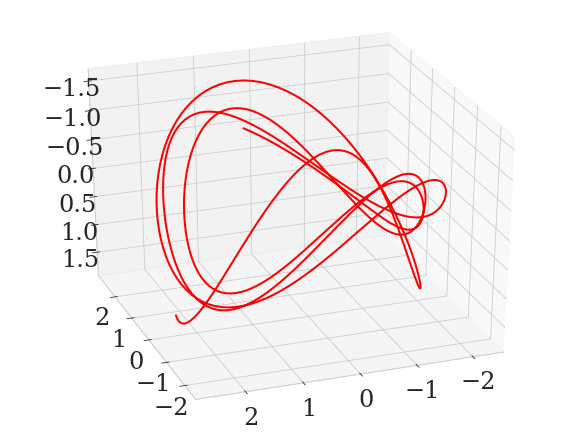
\includegraphics[width=0.6\textwidth]{./images/gyr_tr_2_new.png}}\\
\caption{Траектории в фазовом пространстве для медленной ходьбы}
\label{fg:long_traj}
\end{figure}

\begin{figure}[h!]
\centering
{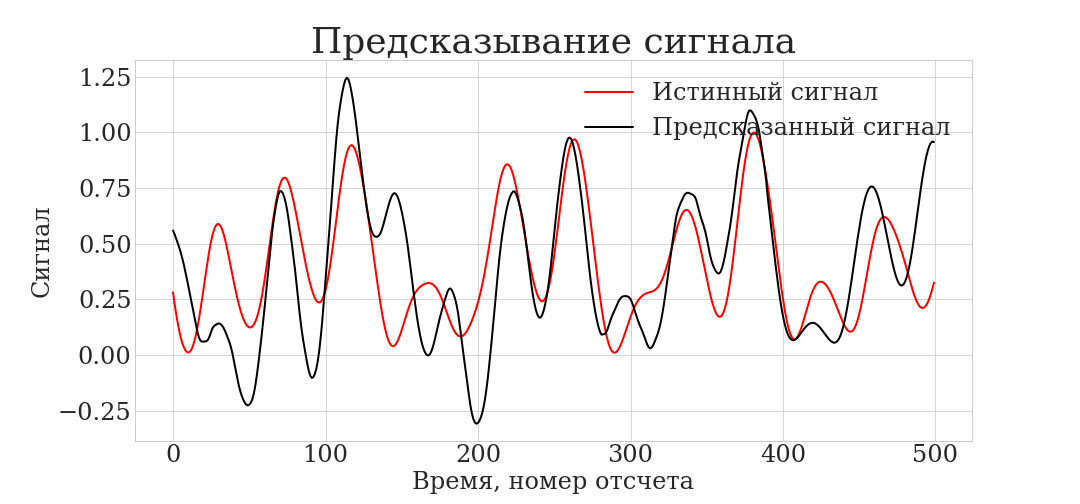
\includegraphics[width=1.1\textwidth]{./images/long_pls_new.png}}
\caption{Предсказание сигнала гироскопа с помощью алгоритма PLS для медленной ходьбы}
\label{fg:long_pred}
\end{figure}

Вычислительный эксперимент проводился на данных \cite{data}.
Целью вычислительного эксперимента является исследование качества предсказания для зависимых и независимых временных рядов. Прогноз строится с помощью метода PLS. Временные ряды проверяются на зависимость с помощью метода сходящегося перекрестного отображения.


В качестве сигналов, которые связаны между собой, были взяты сигналы акселерометра и гироскопа одного мобильного устройства. Были рассмотрены разные типы активности, такие как ходьба различной интенсивности и бег. В качестве сигналов, несвязанных между собой, выбирались сигналы датчиков разных мобильных~устройств.

Для сигналов был выполнен анализ главных компонент с помощью алгоритма SSA(Singular Spectrum Analysis). Для вычислительного эксперимента выбирались первые шесть главных компонент. После этого выполнялась стандартизация и шкалирование временного ряда.

На рисунке \eqref{fg:signal} изображены исходные сигналы акселерометра и гироскопа одного мобильного устройства при ходьбе. На рисунке \eqref{fg:initial_trajectory} изображены фазовые траектории для этих сигналов соответственно. Поиск ближайших соседей на фазовых траекториях проиллюстрирована на рисунке \eqref{fg:CCM}. Окрестности из ближайших точек временного ряда $\bx$ соответствует окрестность точек временного ряда $\by$. Отображение является липшицевым, что подтверждает наличие связи между временными рядами $\bx$ и $\by$, порожденными одной и той же динамической системой $\mathcal{S}$~--- движущимся человеком. На рисунке \eqref{fg:pred} представлен прогноз сигнала гироскопа, полученный с помощью алгоритма PLS.  

Исходные данные, фазовые траектории и прогноз для медленной ходьбы представлены на рисунках \eqref{fg:long_signal}, \eqref{fg:long_traj} и\eqref{fg:long_pred} соответственно.

На рисунке \eqref{fg:uncorr} представлен прогноз сигнала акселерометра в случае двух совершенно несвязанных сигналов. Уже визуально видно, что прогноз в этом случае сильно проигрывает случаю связанных сигналов.


Для каждой пары истинного сигнала и предсказанного сигнала подсчитывалась среднеквадратичная ошибка MSE. Результаты представлены в таблице 1. Ошибка прогноза для случая двух несвязанных сигналов значительно превышает значение ошибки для случая связанных сигналов.

Проведен анализ среднеквадратичной ошибки прогноза от числа компонент в алгоритме PLS. На рисунке \eqref{fg:error_corr} проиллюстрирована зависимость ошибки MSE от числа компонент для случая связанных сигналов. С увеличением числа компонент значение ошибки прогноза падает. Оптимальное число компонент равно примерно 17-ти. На рисунке \eqref{fg:error_uncorr} представлен аналогичный график для случая двух несвязанных сигналов. Ошибка прогноза растет с увеличением числа компонент. Следует выбирать около трех компонент. 

Рассчитаны коэффициенты корреляции Пирсона и Спирмена между истинными и предсказанными сигналами.
Временные ряды разбивались на 10 блоков, на каждом из которых  был рассчитан коэффициенты корреляци. Результаты приведены в таблице 3 и 4. Номер эксперимента соответствует описанию из таблицы 1 соответственно. По результатам вычислений Коэффициенты корреляции ниже в случае несвязанных сигналов.

Еще один эксперимент проводился для пары сигналов, которые сдвигались друг относительно друга на несколько отсчетов. Интервал сдвига меняется в пределах от 50 до 450. В таблице 2 приведены значения среднеквадратичной ошибки для данного эксперимента. Результаты показывают, что с увеличением интервала сдвига возрастает значение ошибки MSE.


\begin{table}[bhtp]
	\centering
	\caption{Среднеквадратичное отклонение между истинными показаниями устройств и предсказаниями, полученными с помощью алгоритма PLS}
	\label{tbl:methods}
	\begin{tabular}{l|l|l|l|c}
		\hline
	Номер экспмеримента	& Датчики & Прибор & Тип движения & MSE \\
		\hline
	1 & Акселерометр + гироскоп & один & ходьба & 0.006 \\
	2 & Акселерометр + гироскоп & один & медленная ходьба & 0.069  \\
	3 &	Акселерометр + акселерометр & разные & ходьба & 0.997  \\
	4 &	Акселерометр + гироскоп & один & бег & 0.027  \\
	5 &	Акселерометр + гироспкоп & один & быстрая ходьба & 0.024  \\

		\hline   
	\end{tabular}
\end{table}

\begin{table}[bhtp]
	\centering
	\caption{Предсказание сигнала гироскопа по сигналу акселерометра одного мобильного устройства при ходьбе с помощью алгоритма PLS, сигналы сдвинуты относительно друг друга}
	\label{tbl:methods}
	\begin{tabular}{l|c}
		\hline
		Величина сдвига & MSE \\
		\hline
	    0 отсчетов & 0.0061 \\
		50 отсчетов & 0.0054  \\
		100 отсчетов & 0.0081  \\
		150 отсчетов & 0.0086  \\
		200 отсчетов & 0.0094  \\
		250 отсчетов & 0.0097  \\
		300 отсчетов & 0.0116   \\
		350 отсчетов & 0.0118  \\
		400 отсчетов & 0.0126  \\
		450 отсчетов & 0.0152  \\
		

		\hline   
	\end{tabular}
\end{table}

\begin{table}[bhtp]
	\centering
	\caption{Коэффициент корреляции Пирсона между истинным и предсказанным сигналами}
	\label{tbl:methods}
	\begin{tabular}{l|l|l|l|l|l|l|l|l|l|c}
		\hline
		Номер эксперимента & 1 & 2 &  3 &  4 & 5 &  6 &  7 & 8 &  9 & 10 \\
		\hline
	    1 & 0.77 & 0.80 & 0.73 & 0.63 & 0.70 & 0.88 & 0.67 & 0.70 & 0.76 & 0.62 \\
		2 & -0.23 & 0.92 & 0.74 & -0.12  & 0.71 & 0.89 & 0.92 & 0.91 & -0.24 & -0.39  \\
		3 & 0.32 & 0.10 & 0.03 & -0.10 & -0.17 & 0.20 & 0.65 & -0.66 & 0.34 & 0.37 \\
		4 & 0.80 & 0.75 & 0.66 & 0.50 & 0.48 & 0.47 & 0.71 & 0.68 & 0.54 & 0.37  \\
		5 & -0.05 & 0.53 & -0.04 & -0.44 & 0.27 & -0.18 & -0.24 & -0.30 & -0.10 & 0.74  \\
		\hline   
	\end{tabular}
\end{table}

\begin{table}[bhtp]
	\centering
	\caption{Коэффициент корреляции Спирмена между истинным и предсказанным сигналами}
	\label{tbl:methods}
	\begin{tabular}{l|l|l|l|l|l|l|l|l|l|c}
		\hline
		Номер эксперимента & 1 & 2 &  3 &  4 & 5 &  6 &  7 & 8 &  9 & 10 \\
		\hline
	    1 & 0.74 & 0.77 & 0.71 & 0.51 & 0.64 & 0.83 & 0.60 & 0.51 & 0.69 & 0.63 \\
		2 & -0.24 & 0.90 & 0.66 & -0.16  & 0.74 & 0.83 & 0.86 & 0.89 & -0.02 & -0.37  \\
		3 & 0.31 & 0.13 & -0.10 & -0.11 & -0.11 & 0.21 & 0.45 & -0.51 & 0.30 & 0.09 \\
		4 & 0.81 & 0.78 & 0.51 & 0.53 & 0.42 & 0.48 & 0.72 & 0.78 & 0.48 & 0.30  \\
		5 & 0.04 & 0.50 & -0.08 & -0.57 & 0.21 & -0.22 & -0.29 & -0.18 & 0.02 & 0.74  \\
		\hline   
	\end{tabular}
\end{table}

Вычислительный эксперимент подтверждает теоретический факт о том, что метод PLS является частным случаем метода перекрестных отображений Сугихары. 

Результаты эксперимента позволяют ответь на вопрос: достаточно ли из двух сигналов, акселерометра и гироскопа, какого-либо одного из них. Этого можно достичь в случае хорошего качества восстановления одного сигнала по второму. В данном эксперименте по сигналу акселерометра восстанавливается сигнал гироскопа с помощью алгоритма PLS.

Все результаты вычислительного эксперимента воспроизводимы по ссылке \cite{code}.


\section{Заключение}

В данной работе исследована связь между методами канонического корреляционного анализа и методами сходящихся перекрестных отображений Сугихары. Сформулирована теорема о том, что методы канонического корреляционного анализа являются частным случаем метода Сугихары. Справедливость теоремы показана на частном примере для метода PLS. 

В работе проведен анализ литературы и обзор современных методов в области канонического корреляционного анализа и методов Сугихары.

Проведен вычислительный эксперимент по построению прогноза сигналов с датчиков движения человека. Решена задача учета структуры временных рядов. Предложенный подход объединяет метод PLS и метод сходящегося перекрестного отображения. Исследована среднеквадратичная ошибка прогноза, а также корреляция Пирсона и Спирмена между истинным и предсказанным сигналами. Показано, что наличие зависимости между временными рядами улучшает качество прогноза. 

В продолжении данной работы планируется исследование справедливости гипотезы в теоретической постановке, а также рассмотреть другие методы канонического корреляционного анализа.

\addcontentsline{toc}{section}{Литература}

\bibliographystyle{unsrt}
\bibliography{biblio}
\nocite{*}
\newpage
\section*{Список основных обозначений}
\addcontentsline{toc}{section}{Список основных обозначений}
\noindent 
$\mathcal{S}$~--- динамическая система\\
$\mathbb{M}$~--- пространство состояний динамической системы\\
$f_M$~--- динамика системы\\
$\bM$~--- многообразие\\
$\phi$~--- диффеоморфизм вложения\\
$\alpha$~--- функция наблюдений\\
$\bx = \{ x_1,\dots, x_{N_1}\}$~--- исходный временной ряд\\
$\by = \{ y_1,\dots, y_{N_2}\}$~--- целевой временной ряд\\
$\mathbb{X}$~--- фазовое пространство исходной переменной \\
$\mathbb{Y}$~--- фазовое пространство целевой переменной \\
$\mathbf{X} = [\bx_1, \dots, \bx_{k_1}]^{\T} $~--- исходная матрица \\
$\mathbf{Y} = [\by_1, \dots, \by_{k_2}]^{\T} $~--- целевая матрица  \\
$\bM_X$~--- аттрактор исходной переменной\\
$\bM_Y$~--- аттрактор целевой переменной\\
$\mathcal{F}$~--- прогностическая модель \\
$\bw$~--- параметры модели \\
$\mathcal{L}(\bw, \widehat{\by}, \by)$~--- функция ошибки прогностической модели \\
$h$~--- горизонт прогнозирования\\
$m$~--- количество шагов прогноза\\
$\mathbf{\Theta}$~--- матрица весов линейной зависимости\\
$\boldsymbol{\varepsilon}$~--- вектор ошибок линейной зависимости\\
$L(\mathbf{\Theta}, \bX, \bY)$~--- функция ошибки линейной зависимости\\
$\bP$~--- матрица перехода из латентного пространства в исходное\\
$\bQ$~--- матрица перехода из латентного пространства в целевое\\
$\mathbf{T}$, $\mathbf{U}$~--- матрицы, описывающие латентно-согласованные пространства \\
$\varphi$~--- отображение фазовых пространств\\
$\rho_{\mathbb{X}},\, \rho_{\mathbb{Y}}$~--- метрики в пространствах $\mathbb{X}$ и $\mathbb{Y}$\\
$C$~--- константа Липшица\\
$U_k(\bx_0)$~--- окрестность $k$ ближайших соседей точки $\bx_0$\\
$R(U_k(\bx_0))$~--- среднее расстояние от точки $\bx_0$ до $k$ ближайших соседей\\
$J$~---  метрическая функция близости


\end{document}
